
\section{Implementační úkoly}

Jednotlivé funkce byly naimplementovány. Funkce \code{fit\_circle(method)} umí pracovat se dvěma metodami ze zadání.

\section{Teoretické úkoly}

\subsection{Vyšetření grafu funkce}

\begin{figure}[H]
    \centering
    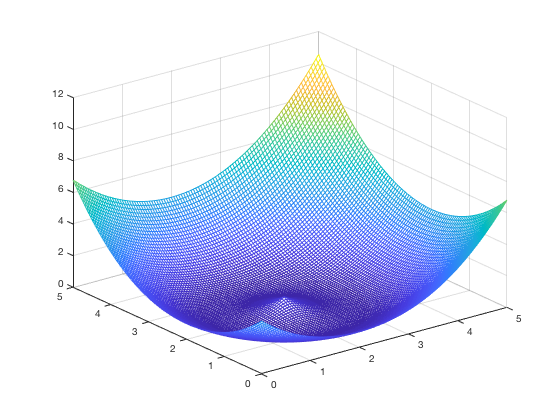
\includegraphics[width=0.8\textwidth]{../1point.png}
    \caption{Graf závislosti vzdálenosti bodu na poloze středu kružnice s jednotkovým poloměrem}
\end{figure}

\begin{figure}[H]
    \centering
    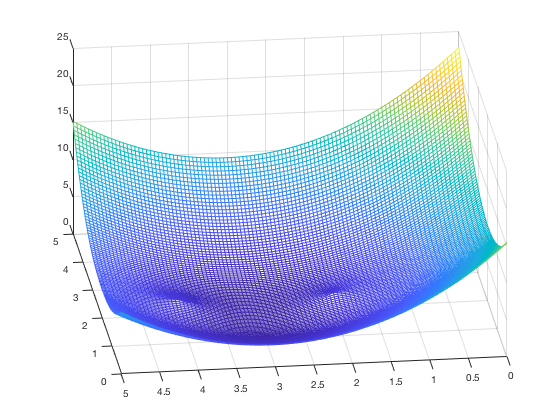
\includegraphics[width=0.7\textwidth]{../2points.png}
    \caption{Graf závislosti vzdálenosti dvou bodů na poloze středu kružnice s jednotkovým poloměrem}
\end{figure}

\begin{figure}[H]
    \centering
    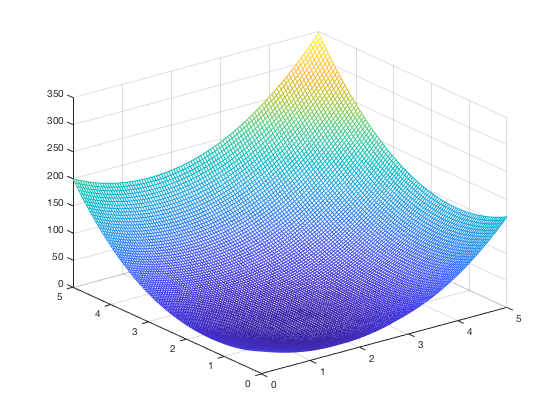
\includegraphics[width=0.7\textwidth]{../20points.png}
    \caption{Graf závislosti vzdálenosti dvaceti bodů na poloze středu kružnice s jednotkovým poloměrem}
\end{figure}

\begin{itemize}
    \item Je funkce \( f \) všude diferencovatelná?

    Není diferencovatelná v bodě, který je shodný se středem kružnice.

    \item Má jedno nebo více lokálních minim?

    Funkce má určitě více lokálních minim. Např. pro střed kružnice je minimem celá kružnice.
\end{itemize}

\subsection{Vyšetření algoritmů}

Po pár provedených pokus jsem došel k závěru, že Gauss-Newtonova metoda diverguje poměrně snadno. Stačí kružnici nastavit poloměr příliš velký nebo malý a umístit střed kružnici mimo konvexní obal bodů. Na druhé straně Levenberg-Marquadtovův algoritmus našel minimum na mém omezeném příkladu pokaždé. Díky tomu se jeví jako lepší pro hledání minima funkce \( f \lr{\bf{x}} \).

\subsection{Více lokálních minim}

\begin{figure}[H]
    \centering
    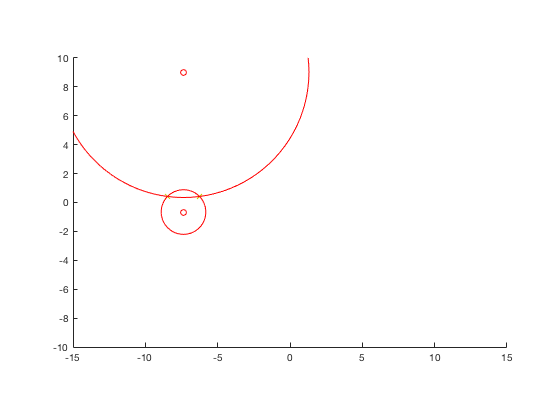
\includegraphics[width=0.7\textwidth]{../2minims.png}
    \caption{Graf dvou různých minim pro jeden datový set}
\end{figure}

Nejjednodušší je použít dva body. Pokud těmito dvěma body proložíme přímku, tak na jedné straně přímky se bude nacházet střed kružnice v prvním lokálním minimu a na druhé straně druhý.

Lepší bude použít tu kružnici, jejíž poloměr je menší, možná zaokrohlouvací chyba během výpočtu bude menší. Současně bude lepší i v případě, že výsledek bude použit jako vstup do nějakého dalšího algoritmu.
